The aim of this procedure is the estimation of the median spectral acceleration value $\hat{S}_a$, that brings the structure to the attainment of a set of damage states, and the corresponding dispersion beta $\beta_{S_a}$, the parameters needed for the mathematical representation of fragility in equation \ref{eq:fragility-definition}. The aim is achieved making use of a R-$\mu$-T relationship, between the reduction factor R, the ductility $\mu$ and period T, which is based on the work of Dolsek and Fajfar (2004). The R-$\mu$-T-based procedure presented herein is applicable to any kind of multi-linear capacity curve, and it is suitable for single building fragility curve estimation, as described in section \ref{subsubsec:single-building-DF}. However the fragility curves derived for single buildings can be combined in a unique fragility curve, which considers the inter-building uncertainty, as described in section \ref{subsubsec:multiple-building-DF}.

\subsubsection{Single Building Fragility and Vulnerability function}
\label{subsubsec:single-building-DF}
The spectral value at each damage state threshold \textit{ds} $\hat{S}_{a,ds}$ is found from the roof displacement limit state for that \textit{ds} $\hat{d}_{roof, ds}$, as explained in C$_{R}$-based procedure and reported by the following equation:

\begin{equation}
\hat{S}_{a,ds}(T_1) = \frac{4 \pi^2}{\hat{C}_R T^2 \Gamma_1 \Phi_1} \hat{d}_{roof, ds}
\label{eq:basic_DF}
\end{equation}

The value of C$_R$, the ratio between the inelastic and the elastic spectral displacement, is found from the following equation:

\begin{equation}
\hat{C}_{R} = \frac{\mu_{ds}}{R_{ds}}
\label{eq:Cr_DF}
\end{equation}

where $\mu_{ds}$ and $R_{ds}$ are the ductility level and the reduction factor at the attainment of \textit{ds}. According to the results of an extensive parametric study using three different sets of recorded and semi-artificial ground motions, Dolsek and Fajfar (2004) related the ductility demand $\mu$ and reduction factor R through the following formula:

\begin{equation}
\label{eq:mu_DF}
\mu = \frac{1}{c} (R-R_{0})+\mu_{0}
\end{equation}

In the proposed model $\mu$ is linearly dependent on R within two reduction factor intervals. The parameter c defines the slope of the R–$\mu$ relation, and depends on the initial period of the system T, the ratio r$_{u}$, the reduction factor R and the corner periods T$_{c}$ and T$_{d}$. T$_{c}$ and T$_{d}$ are the corner periods between the constant acceleration and constant velocity part of the idealized elastic spectrum, and between the constant velocity and constant displacement part of the idealized elastic spectrum respectively.\\

Given the parameters of the multilinear pushover curves (R$_{\mu_{c}}$, $\mu_{c}$, r$_{u}$) and T, the median R - $\mu$ curve can be constructed using the aforementioned relationship. 
The relationship between the 16$^{th}$ and 84$^{th}$ fractiles of $\mu$ and R needs to be derived using the equations from Ruiz-Garcia and Miranda instead, given that Dolsek and Fajfar do not provide estimates of the dispersion of R. This is done as in the C$_R$-based procedure by computing $\beta_{\theta d}$ for a number of R with eq. \ref{eq:beta_eq_RGM}, and obtaining from this value the 16$^{th}$ and 84$^{th}$ fractiles of $\mu$ ($\mu_{16\%}$ and $\mu_{84\%}$), according to the Equations \ref{eq:mu16-beta} and \ref{eq:mu84-beta}.\\

For each $\mu_{ds}$ the corresponding $R_{50\%}$, $R_{16\%}$, and $R_{84\%}$ values are found interpolating the aforementioned curves, and converted into $\hat{S}_{a,ds}$ and $\beta_{S_{a d}}$ according to equations \ref{eq:SaR} and \ref{eq:betaR}.

If dispersion due to uncertainty in the limit state definition $\beta_{\theta c}$ is different from zero it can be combined with the record-to-record dispersion either in a simplified way or with a Monte Carlo sampling procedure similar to what is done in section \ref{subsubsec:single-building}.\\

In the simplified method the dispersion of $S_a$ due to uncertainty in the damage state threshold $\beta_{S_{a c}}$  can be found converting the dispersion on the damage threshold $\beta_{\theta c}$, as explaind in section \ref{subsubsec:single-building} and reported in the following equation:

\begin{equation}
\beta_{S_{a c}} = \frac{1}{b} \beta_{\theta c}
\label{eq:betasc_DF}
\end{equation}

In order to derive the b values, which represent the slope of the R-$\mu$ relation in the log-space, a further step needs to be made, because the R-$\mu$-T is suggested by the authors as conservative, since it is not based on the median but on the mean $\mu$ given R. An attempt was made to correct it reducing the median R curve by 15\%, $\hat{R}_{corrected}$, as shown in equation \ref{eq:Rcorrected}, and extrapolating the corresponding $\hat{\mu}_{corrected}$.

\begin{equation}
\hat{R}_{corrected}=0.85\hat{R}
\label{eq:Rcorrected}
\end{equation}
\begin{equation}
b = \frac{ln(\hat{\mu}_{corrected})}{ln(\hat{R}_{corrected})}
\label{eq:bcorrected_DF}
\end{equation}

Finally the dispersion of $S_a$ due to record-to-record variability, can be combined with the dispersion of $S_a$ due to uncertainty in the damage state threshold, as in the following equation:

\begin{equation}
\beta_{S_a} = \sqrt{\beta_{S_{a c}}^2+\beta_{S_{a d}}^2}
\label{eq:betatot_DF}
\end{equation}

In the Monte Carlo approach different values of ductility limit state are sampled from the lognormal distribution with median the median value of the ductility limit state, and dispersion the input $\beta_{\theta c}$.
For each of these ductilities the corresponding $R_{50\%}$, $R_{16\%}$, and $R_{84\%}$ values are found interpolating the aforementioned curves, and converted into $\hat{S}_{a,ds}$ and $\beta_{S_{a d}}$ according to Equations \ref{eq:SaR} and \ref{eq:betaR}.

MC random S$_a$ for each of the MC sampled ductility limit states are computed using $\hat{S}_{a,ds}$ and $\beta_{S_{a d}}$, and their median and dispersion are estimated. These parameters constitute the median $\hat{S}_{a,ds}$ and the total dispersion $\beta_{S_a}$ for the considered damage state. The procedure is repeated for each damage state.

To derive a discrete vulnerability function at certain intensity measure levels, the input damage-to-loss factors are applied to the probability of occurance of each damage state, extracted from the probability of exceedance of each damage state described by the fragility function.
If dispersion due to uncertainty in the limit state is different from zero a vulnerability function is derived for the MC sets of sampled ductility limit states. It results in MC loss ratios for each defined intensity measure levels. Finally a lognormal distribution of the loss ratios is assumed at each iml and the vulnerability curve is defined at each iml by the mean and the standard deviation of all the computed loss ratios.

\subsubsection{Multiple Building Fragility and Vulnerability function}
\label{subsubsec:multiple-building-DF}
 If multiple buildings have been input to derive fragility function for a class of buildings all $\hat{S}_{a, blg}$ and $\beta_{S_a, blg}$ are combined in a single lognormal curve as described in section \ref{subsubsec:multiple-buildings}. The same holds for vulnerability function, as described in the same section.

\subsubsection{Inputs}
The data the user needs provided and the their format is described in section \ref{subsubsec:InputSpo2ida}

\subsubsection{Calculation Steps} 
The overall workflow of R-$\mu$-T-based procedure is summarised in this section and represented in Figure \ref{fig:Cr_workflow} for the case of a single building fragility/vulnerability function. 

\begin{figure}[!htbp]
\centering
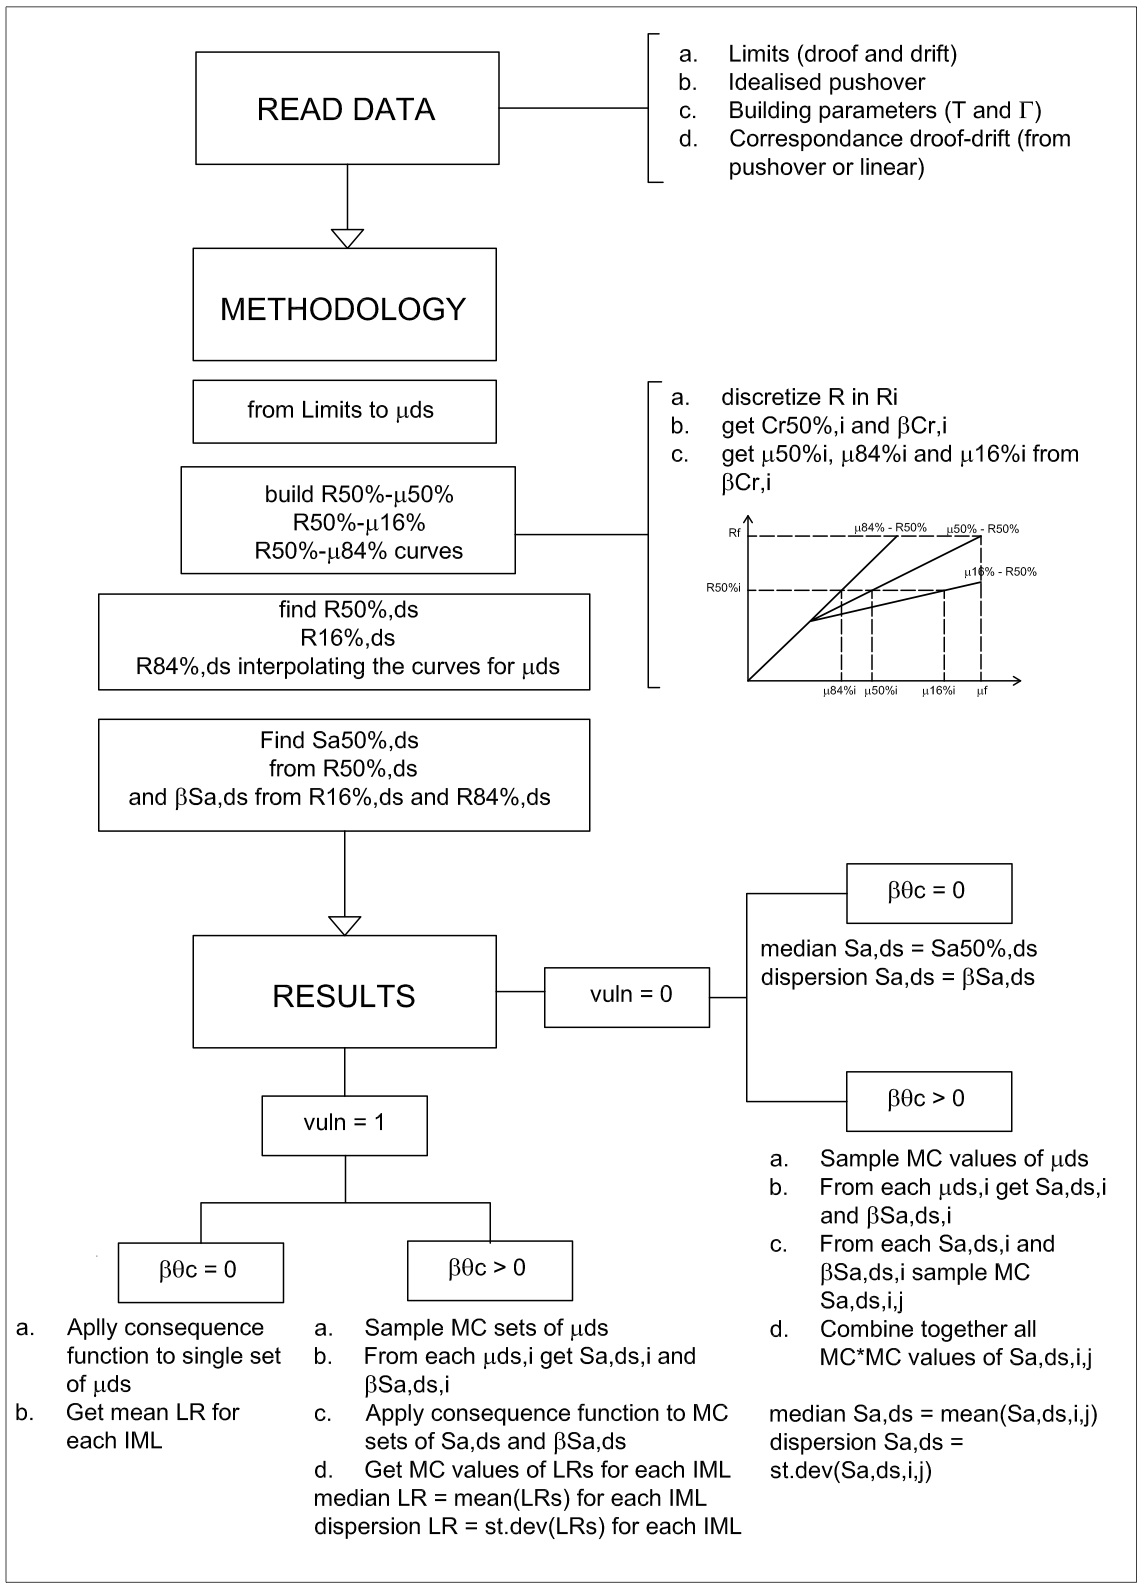
\includegraphics[width=15cm]{./figures/Cr-WorkFlow.jpg}
\caption{C$_R$-based procedure workflow.}
\label{fig:Cr_workflow}
\end{figure}

The option \textit{an\_type} must be set equal to 2 and the option \textit{in\_type} according to the input at disposal. The corresponding inputs should follow the requirements described in section \ref{subsubsec:InputSpo2ida}. At this point the code proceeds with the following steps:\\

\begin{enumerate}
\item \textbf{Process Inputs within \textit{read\_data}  function}\\

\begin{enumerate}
\item If \textit{in\_type} = 0, the roof displacement at each limit state and the idealised pushover curve parameters are extracted from \textit{displacement\_profile.csv} and \textit{idealised\_curve.csv} respectively.
\item If \textit{in\_type} = 1 the results from a pushover analysis are extracted from \textit{displacements\_pushover.csv} and \textit{reactions\_pushover.csv} and drift limit states from {limits.csv}. The idealised pushover curve is then derived in the \textit{idealisation} function, where the idealisation process is conducted according to the Gem Analytical Vulnerability Guidelines.\\
\end{enumerate}

Period, modal participation factor, number of buildings constituting the building class, importance factor (weight) of the each building within the class, average period of the class and the ratio $S_a(T_{av})/S_a(T_{blg})$ are also returned by the function \textit{read\_data} .\\

\item \textbf{Fragility curve methodology}\\
The parameters extracted are used in the \textit{DF\-fragility} function, within the \textit{fragility\_process} function, to derive ductility levels $\mu_{ds}$, median spectral acceleration $\hat{S}_{a,ds}$ and the total dispersion $\beta_{S_a}$ at each limit state through the following steps:

\begin{enumerate}

\item The idealised MDoF system is transformed into an equivalent SDoF system, using $\Gamma_1$.

\item Ductility levels $\mu_{ds}$ corresponding to each damage threshold, are defined.

\item Median $\mu$ - R relationship is computed using Equation \ref{eq:mu_DF}.

\item $\mu_{16\%}$ - $R_{50\%}$ and $\mu_{84\%}$ - $R_{50\%}$ relationships are computed as in C$_R$-based procedure.

\item $R_{50\%}$, $R_{16\%}$ and $R_{84\%}$ is computed for the ductility limit states $\mu_{ds}$, interpolating the aforementioned R - $\mu$ curves.

\item $\hat{S}_{a,ds}$ and the corresponding dispersion $\beta_{S_{a d}}$ due to record-to-record variability are computed using eq. \ref{eq:SaR} and \ref{eq:betaR} for each limit state.

\item If dispersion due to uncertainty in the limit state $\beta_{\theta c}$ is different from zero, different ductility limit states are sampled for each median ductility level $\mu_{ds}$. For each sampled ductilities the corresponding $\hat{S}_{a,ds}$ and $\beta_{S_{a ds}}$ are found as described in steps from (d) to (f), and MC random S$_a$ for each of the MC sampled ductility limit states are computed using $\hat{S}_{a,ds}$ and $\beta_{S_{a d}}$.\\

\end{enumerate}

\item \textbf{Fragility curve results}\\
If number of buildings = 1\\
\begin{enumerate}
\item If \textit{vuln} = 0
the final values of median and dispersion of the fragility curves, $\hat{S}_{a,ds}$ and $\beta_{S_a}$, are computed as the mean and the standard deviation of the MC$^2$ samples of S$_a$, if many $\mu_{ds}$ were sampled at step 2.g, otherwise they correspond to the $\hat{S}_{a,ds}$ and $\beta_{S_{a d}}$, including only record-to-record variability, obtained at step 2.f.

All $\hat{S}_{a, ds}$ are converted to mean $\mu_{ln(S_{a, ds})}$. Mean $\mu_{ln(S_{a})}$ and total dispersion $\beta_{S_a}$ are then converted to logarithmic mean $\mu_{S_a}$ and logarithmic covariance $cov_{S_a}$, according to equations \ref{eq:median-to-mean} and \ref{eq:dispersion-to-standard} respectively.

Fragility curves for the building are displayed if the variable \textit{plotflag}[2] = 1, and logarithmic $\mu_{S_a}$ and $cov_{S_a}$ are exported in the \textit{outputs} folder.

\item 
If \textit{vuln} =1
For each intensity measure level defined in the variable \textit{iml} MC values of loss ratio LRs are defined for the MC sets of $\mu_{ds}$, if many values were sampled to account for uncertainty in the damage criteria at step 2.f, using the \textit{damage\_to\_loss} function. Mean and standard deviation of LRs(iml), $\mu_{LR}$ and $\beta_{LR}$, are computed. If $\beta_{\theta c}$= 0 a single set of $\mu_{ds}$ is considered, resulting in no uncertainty in the LR for each iml.\\

Vulnerability curve for the building is displayed if the variable \textit{plotflag}[3] = 1, and $\mu_{LR}$ and $cov_{LR}$ at each iml are exported in the \textit{outputs} folder.\\

\end{enumerate}

If number of buildings > 1\\
\begin{enumerate}
\item If \textit{vuln} = 0
the final values of median and dispersion of the fragility curves, $\hat{S}_{a,ds}$ and $\beta_{S_a}$, are computed as the mean and the standard deviation of the MC$^2$ samples of S$_a$, if many $\mu_{ds}$ were sampled at step 2.g, otherwise they correspond to the $\hat{S}_{a,ds}$ and $\beta_{S_{a d}}$, including only record-to-record variability, obtained at step 2.f.

All $\hat{S}_{a, ds, blg}(T_1)$ are converted to mean $\mu_{ln(S_{a, ds, blg})}(T_1)$ and then to the intensity measure in common with the rest of the buildings, $\mu_{ln(S_{a, ds, blg}(T_{av}))}$, according to eq. \ref{eq:Sa(Tav)}.\\
The $\mu_{ln(S_{a, ds, blg}(T_{av}))}$ are finally combined in a single lognormal curve for the building class, as described in section \ref{subsubsec:multiple-buildings}. 

Mean $\mu_{ln(S_{a})}$ and total dispersion $\beta_{S_a}$ are then converted to logarithmic mean $\mu_{S_a}$ and logarithmic covariance $cov_{S_a}$, according to equations \ref{eq:median-to-mean} and \ref{eq:dispersion-to-standard} respectively.

Fragility curves for the class of buildings are displayed if the variable \textit{plotflag}[2] = 1, and logarithmic $\mu_{S_a}$ and $cov_{S_a}$ are exported in the \textit{outputs} folder.

\item 
If \textit{vuln} =1
all $\hat{S}_{a, ds}(T_1)$ for each building are converted to mean $\mu_{ln(S_{a, ds})}(T_1)$ and then to the intensity measure in common with the rest of the buildings, $\mu_{ln(S_{a, ds, blg}(T_{av}))}$, according to eq. \ref{eq:Sa(Tav)}.

For each intensity measure level defined in the variable \textit{iml} MC values of loss ratio LRs are defined for the MC sets of $\mu_{ds}$, if many values were sampled to account for uncertainty in the damage criteria at step 2.f, using the \textit{damage\_to\_loss} function. Mean and standard deviation of LRs(iml), $\mu_{LR}$ and $\beta_{LR}$, are computed. If $\beta_{\theta c}$= 0 a single set of $\mu_{ds}$ is considered, resulting in no uncertainty in the LR for each iml.\\

The $\mu_{LR, iml, blg}$ are finally combined in a single mean and standard deviations, as described in section \ref{subsubsec:multiple-buildings}. Vulnerability curve for the class of buildings is displayed if the variable \textit{plotflag}[3] = 1, and $\mu_{LR}$ and $cov_{LR}$ at each iml are exported in the \textit{outputs} folder.

\end{enumerate}

\end{enumerate}

